\section{Lektion 20-02-2018}

\begin{enumerate}
	\item Komponenter og systemer
	\item Resonanskredsløb
	\item Tabsfrie komponenter
	\item Impedans transformation
	\item Filter design
	\item Frekvens og impedans skalering
\end{enumerate}

\begin{mdframed}[style=exampledefault]
	\begin{itemize}
		\item \textbf{Pensum:} CB, Ch 1+2+3
		\item \textbf{Opgaver:} Uge 3-1, Uge 3-2
	\end{itemize}
\end{mdframed}

\subsection{Komponenter}
Komponenters egenskaber, modstande, kondensatorer og induktorer ved radiofrekvenser og hvordan det vedrører kredsløbsdesign. De mest enkle komponenter af ethvert system undersøges ved radiofrekvenser.
\begin{itemize}
	\item Wire (diameter, længde)
	\begin{itemize}
		\item Skin Effect
		\begin{itemize}
			\item As frequency is increased, an increased magnetic field at the center of the conductor presents an impedance to the charge carriers, thus decreasing the current density at the center of the conductor and increasing the current density around its perimeter.
			\item It occurs in all conductors including resistor leads,
			capacitor leads, and inductor leads.
		\end{itemize}
		\item Skin Depth
		\begin{itemize}
			\item The depth into the conductor at which the charge-carrier current density falls to $\frac{1}{e}$, or 37\% of its value along the surface.
			\item Is a function of the frequency and the permeability and conductivity of the medium.
			\item Results in a net increase in	the ac resistance of the wire.
		\end{itemize} 
		\item Straight-Wire Inductors
		\begin{itemize}
			\item Self-Inductance happens when current in the conductor is an alternating current. A magnetic field is alternately expanding
			and contracting and, thus, producing a voltage on the wire which
			opposes any change in current flow.
		\end{itemize}
	\end{itemize}
\end{itemize}

\begin{equation}
L = 0.002\,l\left[2.3\log\left(\dfrac{4l}{d}\right)-0.75\right] \si{\micro\henry}
\end{equation}
\begin{description}
	\item[L] inductance in \si{\micro\henry}
	\item[l] length of wire in \si{\centi\meter}
	\item[d] diameter of wire in \si{\centi\meter}
\end{description}

\begin{itemize}
	\item Resistors
	\begin{itemize}
		\item Resistor Equivalent Circuit
		\begin{itemize}
			\item \textit{R} is the resistor value itself.
			\item \textit{L} is the lead inductance.
			\item \textit{C} is a combination of parasitic capacitances
			which varies from resistor to resistor.
		\end{itemize}
		\item Resistor Types
		\begin{itemize}
			\item \textit{Carbon-composition resistors} consists of densely packed dielectric particulates or carbon granules.
			Between each pair there is a very small parasitic capacitor.
			\item \textit{Wirewound resistors} tend to exhibit widely varying
			impedances over various frequencies. 
			\begin{itemize}
				\item The inductor L, is much larger for a wirewound resistor than for a carbon-composition resistor.
			\end{itemize}
			\item \textit{Metal-film resistors} has the best characteristics
			over frequency since the values of the	individual parasitic elements in the equivalent circuit decrease.
			\begin{itemize}
				\item At very high frequencies, and with low-value resistors (under \SI{50}{\ohm}), lead	inductance and skin effect may become noticeable.
			\end{itemize}
			\item \textit{Thin-film chip resistors} offers very little parasitic reactance at frequencues from DC to \SI{2}{\giga\hertz}.
		\end{itemize}
	\end{itemize}
\end{itemize}

\begin{figure} [H]
	\centering
	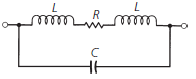
\includegraphics[width=0.4\linewidth]{graphics/15.png}
	\caption{Resistor equivalent circuit.}
	\label{fig:15}
\end{figure}

\begin{equation}
X_L = \omega L
\end{equation}

\begin{equation}
X_C = \dfrac{1}{\omega C}
\end{equation}

\begin{itemize}
	\item Capacitors
	\begin{itemize}
		\item Parallel-Plate Capacitor
		\begin{itemize}
			\item Two conducting surfaces separated by an insulating material or dielectric.
			\item When a potential difference exists between the conductors a capacitor storage a charge. 
			\item[] $C = \dfrac{Q}{V}$
			\begin{itemize}
				\item \textit{C} is capacitance in farads
				\item \textit{Q} is charge in coulombs
				\item \textit{V} is voltage in volts
			\end{itemize}
		\item If the area (\textit{A}) of each metal plate, the distance
		(\textit{d}) between the plate, and the permittivity ($\epsilon$) of the dielectric material in farads/meter are known, the capacitance of a
		parallel-plate capacitor can be found.
		\end{itemize}
	\end{itemize}
\end{itemize}

\begin{equation}
C = \dfrac{0.2249 \epsilon A}{d \,\epsilon_0} \si{\pico\farad}
\end{equation}

\begin{itemize}
	\item[]	
	\begin{itemize}
		\item Real-World Capacitors
		\begin{itemize}
			\item The dielectric’s characteristics determine the voltage levels and the temperature extremes at	which the device may be used.
			\item As the frequency of operation increases, the lead
			inductance becomes important. Finally, at $F_r$, the inductance
			becomes series resonant with the capacitor. Then, above $F_r$, the
			capacitor acts like an inductor.
		\end{itemize}
	\end{itemize}
\end{itemize}

\begin{figure} [H]
	\centering
	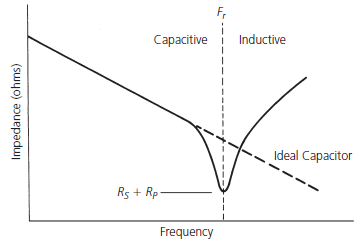
\includegraphics[width=0.65\linewidth]{graphics/16.png}
	\caption{Impedance characteristic vs. frequency.}
	\label{fig:16}
\end{figure}

\begin{itemize}
	\item[] 
	\begin{itemize}
		\item Capacitor Equivalent Circuit
		\begin{itemize}
			\item $C$ equals the capacitance.
			\item $R_s$ is the heat-dissipation loss expressed either as a power factor (PF) or as a dissipation factor (DF).
			\begin{itemize}
				\item[]
				\item[] Power Factor $PF = \cos\phi$ 
				\item[]
				\item In a perfect capacitor, the alternating current	will lead the applied voltage by $90\degree$. This phase angle ($\phi$) will	be smaller in a real capacitor due to the total series resistance ($R_s +R_p$).
				\item[]
				\item[] Dissipation Factor $DF = \frac{ESR}{X_c}\cdot 100\%$
				\item[]
				\item The ratio of AC resistance to the	reactance of a capacitor.
				\item[]
				\item Quality Factor \textit{Q} of a capacitor is the reciprocal of \textit{DF}.
				\item[]
				\item[] $Q = \frac{1}{DF}=\frac{X_c}{ESR}$
				\item[]
				\item[] Effective Series Resistance $ESR = \frac{PF}{\omega C}(1\cdot 10^6)$
				\item[]
				\item Is the AC resistance of a capacitor, a combined equivalent of $R_s$ and $R_p$.  
				\item[]
			\end{itemize}
			\item $R_p$ is the insulation resistance.
			\begin{itemize}
				\item A measure of the amount of DC	current that flows through the dielectric of a capacitor with a voltage applied. No material is a perfect insulator; thus, some	leakage current must flow.
				\item Typically value of \SI{100000}{\mega\ohm} or more.
			\end{itemize}
			\item $L$ is the inductance of the leads and plates.
		\end{itemize}
	\end{itemize}
\end{itemize}

\begin{figure} [H]
	\centering
	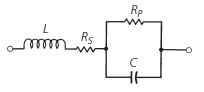
\includegraphics[width=0.4\linewidth]{graphics/17.png}
	\caption{Capacitor equivalent circuit.}
	\label{fig:17}
\end{figure}

\begin{itemize}
	\item[] 
	\begin{itemize}
		\item Capacitor Types
		\begin{itemize}
			\item Ceramic Capacitors
			\begin{itemize}
				\item Vary widely in both dielectric constant \textit{k} and temperature characteristics.
				\item \textit{Rule of thumb is}: "The higher the \textit{k}, the worse is its temperature characteristic."
				\item \textit{Low-k ceramic capacitors} tend to have linear
				temperature characteristic (well suited for
				oscillator, resonant circuit, or filter applications).
				\item \textit{Moderately stable ceramic capacitors} typically vary $\pm15\%$ of their rated capacitance over their temperature range. This variation is typically nonlinear.\\ (used in switching circuits).
				\item \textit{High-K ceramic capacitors} typically termed general-purpose	capacitors. Temperature characteristics are very poor and their capacitance may vary as much as 80\% over various temperature	ranges (used only in bypass applications).
				\item \textit{Chip capacitors} are capacitors that have no leads (specifically intended for RF applications).
			\end{itemize}
			\item Mica Capacitors
			\begin{itemize}
				\item Typically have a dielectric constant \textit{k} of about 6, producing an extremely good temperature characteristic (used extensively in resonant circuits and in filters where PC board area is of no concern).
				\item Are becoming	increasingly less cost effective than ceramic types.
			\end{itemize}
			\item Metalized-Film Capacitors
			\begin{itemize}
				\item Dialectrics of teflon, polystyrene, polycarbonate and paper (used in a number of applications,	including filtering, bypassing, and coupling). 
				\item Polycarbonate, polystyrene, and teflon styles are available in very tight ($\pm2\%$) capacitance tolerances over their entire temperature range.
				\item Typically larger than	the equivalent-value ceramic types.
			\end{itemize}
		\end{itemize}
	\end{itemize}
	\item Inductors
	\begin{itemize}
		\item Inductor Equivalent Circuit
		\begin{itemize}
			\item A wire wound or coiled in	such a manner as to increase the magnetic flux linkage between the turns of the coil which increases the wire's inductance.
			\item Distributed capacitance ($C_d$) 
			\begin{itemize}
				\item Two conductors brought into close proximity but separated by a dielectric, and place a voltage differential between the two, we form a	capacitor.
			\end{itemize}
		\end{itemize}
	\end{itemize}
\end{itemize}

\begin{figure} [H]
	\centering
	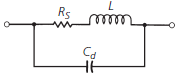
\includegraphics[width=0.4\linewidth]{graphics/18.png}
	\caption{Inductor equivalent circuit.}
	\label{fig:18}
\end{figure}

\begin{itemize}
	\item[] 
	\begin{itemize}
		\item Real-World Inductors
		\begin{itemize}
			\item Initially, at lower frequencies, the inductor's reactance
			parallels that of an ideal inductor. Soon, however, its reactance
			departs from the ideal curve and increases at a much faster
			rate until it reaches a peak at the inductor's parallel resonant
			frequency ($F_r$). 
			\item Above $F_r$ , the inductor’s reactance begins to decrease with frequency and, thus, the inductor begins to look like a capacitor. 
			\item Theoretically, the resonance peak would occur at
			infinite reactance. However, due to the series resistance of the coil, some finite impedance is seen at resonance.
			\item Ratio of an inductor's reactance to its series resistance is
			often used as a measure of the quality of the inductor. The larger
			the ratio, the better is the inductor. 
			\begin{itemize}
				\item Quality Factor $Q = \frac{X}{R_S}$
			\end{itemize}
			\item At low frequencies, the \textit{Q} of an inductor is very good (resistance in the windings is the dc resistance of the
			wire).
			\item As frequency increases, skin effect and winding capacitance begin to degrade the quality of	the inductor.
		\end{itemize}
	\end{itemize}
\end{itemize}


\begin{figure} [H]
	\centering
	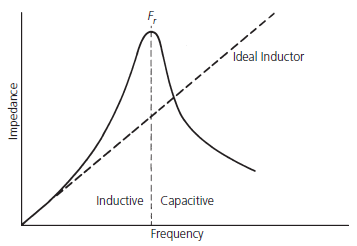
\includegraphics[width=0.6\linewidth]{graphics/19.png}
	\caption{Impedance characteristic vs. frequency for a practical and an
		ideal inductor.}
	\label{fig:19}
\end{figure}

\begin{itemize}
	\item[] 
	\begin{itemize}
		\item[]
		\begin{itemize}
			\item Methods of increasing the \textit{Q} of an inductor and extending its useful frequency range:
			\begin{enumerate}
				\item Use a larger diameter wire. This decreases the AC and
				DC resistance of the windings.
				\item Spread the windings apart. Air has a lower dielectric
				constant than most insulators. Thus, an air gap between
				the windings decreases the interwinding capacitance.
				\item Increase the permeability of the flux linkage path. This
				is most often done by winding the inductor around a
				magnetic-core material, such as iron or ferrite. A coil
				made in this manner will also consist of fewer turns for a
				given inductance.
			\end{enumerate}
		\end{itemize}
		\item Single-Layer Air-Core Inductor Design
		\begin{itemize}
			\item Formula generally used to design single-layer air-core
			inductors \textit{L}.
			\begin{itemize}
				\item Coil length \textit{l} must be greater than $0.67r$. This formula is accurate to within one percent.
			\end{itemize}
		\end{itemize}
	\end{itemize}
\end{itemize}

\begin{equation}
L = \dfrac{0.394 r^2 N^2}{9r + 10l}
\end{equation}

\begin{description}
	\item[r] coil radius in \si{\centi\meter}
	\item[l] coil length in \si{\centi\meter}
	\item[L] inductance in \si{\micro\henry}
\end{description}

\begin{itemize}
	\item[] 
	\begin{itemize}
		\item Magnetic-Core Materials
		\begin{itemize}
			\item Air-Core inductors cannot be used because of their size.
			\item Method of decreasing the size of a coil while maintaining a given inductance:
			\begin{itemize}
				\item Decrease the number of turns while at the same time increasing its magnetic flux density (decreasing the
				"reluctance"). Done by adding a magnetic-core material to the inductor.
			\end{itemize}
			\item[]
			\item Advantages:
			\begin{enumerate}
				\item Smaller size — fewer number of turns needed.
				\item Increased \textit{Q} — fewer turns means less wire resistance.
				\item Variability — obtained by moving the magnetic core in
				and out of the windings.
			\end{enumerate}
			
			\newpage\item Problems:
			\begin{enumerate}
				\item Each core tends to introduce its own losses. Thus, adding
				a magnetic core to an air-core inductor could possibly
				decrease the \textit{Q} of the inductor, depending on the material used and the frequency of operation.
				\item The permeability of all magnetic cores changes with
				frequency and usually decreases to a very small value at
				the upper end of their operating range. It eventually
				approaches the permeability of air and becomes
				"invisible" to the circuit.
				\item The higher the permeability of the core, the more
				sensitive it is to temperature variation. Thus, over wide
				temperature ranges, the inductance of the coil may vary
				appreciably.
				\item The permeability of the magnetic core changes with
				applied signal level. If too large an excitation is applied,
				saturation of the core will result.
			\end{enumerate}
		\end{itemize}
	\end{itemize}
\end{itemize}

\begin{itemize}
	\item Toroids
	\begin{itemize}
		\item Core Inductors Equivalent Circuits
		\begin{itemize}
			\item $R_S =$ resistance of the windings
			\item $R_P =$ losses in the core itself (hysteresis)
			\item[]
			\item To determine the new \textit{Q} of the inductor:
			\begin{itemize}
				\item[] By what factors did the inductance and loss increase?
				\item By adding a toroidal core, inductance will increase
				by a factor of two and its total loss will also increase by a factor	of two - \textit{Q} will remain unchanged.
				\item The additional loss introduced by the core is not constant, but varies (usually increases) with frequency.
			\end{itemize}
		\end{itemize}
	\end{itemize}
\end{itemize}

\begin{figure} [H]
	\centering
	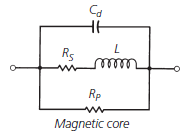
\includegraphics[width=0.4\linewidth]{graphics/20.png}
	\caption{Equivalent circuits for magnetic-core inductor.}
	\label{fig:20}
\end{figure}

\begin{itemize}
	\item[]
	\begin{itemize}
		\item Core Characteristics
		\begin{itemize}
			\item The magnetization curve for a magnetic core indicates the magnetic-flux density (\textit{B}) that occurs in the inductor with a specific magnetic-field intensity (\textit{H}) applied. 
			\begin{itemize}
				\item The ratio of the magnetic-flux density to the magneticfield intensity is called the permeability ($\micro$) of the material.
				\item[] $\micro = \frac{B}{H} \quad webers/ampere\,turn$
				\item[]
				\item As the magnetic-field intensity is increased from
				zero, the magnetic-flux density that links the turns of the inductor increases quite linearly.
				\item A point is reached at which the magnetic-flux
				intensity does not continue to increase at the same rate as the excitation. Any further	increase in excitation may cause saturation to occur $B_{sat}$. The incremental permeability above this	point is the same as air.
			\end{itemize}
			\item Once $B_{sat}$ is known for the core, it is simple to determine whether or not its use in a particular circuit application will cause it to saturate. The in-circuit operational flux density ($B_{op}$) is given by:
		\end{itemize}
	\end{itemize}
\end{itemize}

\begin{equation}
B_{op}=\dfrac{E\cdot 10^8}{(4.44)fNA_e}
\end{equation}

\begin{description}
	\item[$B_{op}$] magnetic-flux density in gauss
	\item[$E$] maximum rms voltage across the inductor
	\item[$f$] frequency in \si{\hertz}
	\item[$N$] number of turns
	\item[$A_e$] effective cross-sectional area of the core in $\si{\centi\meter}^2$
\end{description}

\begin{figure} [H]
	\centering
	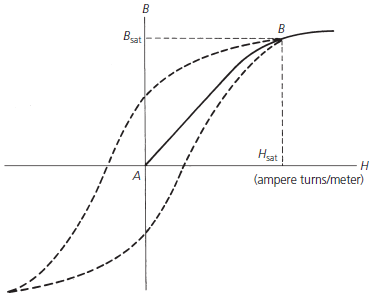
\includegraphics[width=0.6\linewidth]{graphics/21.png}
	\caption{Magnetization curve for a typical core.}
	\label{fig:21}
\end{figure}

\begin{itemize}
	\item[]
	\begin{itemize}
		\item Powdered Iron vs. Ferrite
		\begin{itemize}
			\item In general, no hard and fast rules of ferrite cores versus powdered-iron cores.
			\item Special applications in which one core might outperform another:
			\begin{itemize}
				\item Any application where high RF power levels are involved, iron cores might be the best choice.
				\item Powdered-iron cores tend to yield higher-Q inductors,
				at higher frequencies, than an equivalent size ferrite core making them very useful in narrowband or tuned-circuit applications.
				\item At very low frequencies, or in broadband circuits, ferrite seems to be the	general choice since it has a much higher permeability.
				\item A coil of a given inductance can usually be wound on a
				much smaller ferrite core and with fewer turns than a powdered-iron core and thereby save circuit board area.
			\end{itemize}
		\end{itemize}
		\item Toroidal Inductor Design
		\begin{itemize}
			\item For a toroidal inductor operating on the linear (nonsaturating)	portion of its magnetization curve, its inductance is given by:
		\end{itemize}
	\end{itemize}
\end{itemize}

\begin{equation}
L = \dfrac{0.4\pi N^2 \micro_1 A_c \cdot 10^{-2}}{l_e}
\end{equation}

\begin{description}
	\item[$L$] inductance in \si{\nano\henry}
	\item[$N$] number of turns
	\item[$\micro_1$] initial permeability
	\item[$A_e$] effective cross-sectional area of the core in $\si{\centi\meter}^2$
	\item[$l_e$] effective length of the core in \si{\centi\meter}
\end{description}

\begin{itemize}
	\item[]
	\begin{itemize}
		\item[]
		\begin{itemize}
			\item In order to make calculations easier, most manufacturers have
			combined $\micro_1$, $A_c$, $l_e$, and other constants for a given core into a	single quantity called the inductance index, $A_L$.
		\end{itemize} 
	\end{itemize} 
\end{itemize}

\begin{equation}
L = N^2 A_L \quad \si{\nano\henry}
\end{equation}

\begin{description}
	\item[$L$] inductance in \si{\nano\henry}
	\item[$N$] number of turns
	\item[$A_L$] inductance index in $nanohenries/turn^2$
\end{description}

\begin{itemize}
	\item[]
	\begin{itemize}
		\item[]
		\begin{itemize}
			\item Number of turns to be wound on a given core for a
			specific inductance.
		\end{itemize} 
	\end{itemize} 
\end{itemize}

\begin{equation}
N = \sqrt{\dfrac{L}{A_L}}
\end{equation}

\begin{itemize}
	\item[]
	\begin{itemize}
		\item[]
		\begin{itemize}
			\item A calculated guess of \textit{Q} at low frequencies (\SI{100}{\kilo\hertz}), the \textit{Q} of	the coil would be approximately:
		\end{itemize} 
	\end{itemize} 
\end{itemize}

\begin{equation}
Q = \dfrac{R_p/N^2}{X_p/N^2} = \dfrac{R_p}{X_p}
\end{equation}

\subsection{Resonanskredsløb}
\subsubsection{Tabsfrie komponenter}
\begin{itemize}
	\item Hvis $Z_p$ er en frekvensafhængig impedans (capacitive or inductive reactance), så vil $V_{out}$ også være frekvensafhængig.
	\item Forholdet mellem $V_{out}$ og $V_{in}$ vil udgøre gain/loss i kredsløbet, som også vil være frekvensafhængig. 
\end{itemize}

\begin{equation}
\dfrac{V_{out}}{V_{in}} = 20\log_{10}\dfrac{X_C}{R_s+X_C}
\end{equation}

\begin{description}
	\item[$R_s$] source resistance
	\item[$X_C$] reactance of capacitor
\end{description}

\begin{equation}
X_C=\dfrac{1}{j\omega C}
\end{equation}

\noindent\textit{The loss of this RC circuit	increases as the frequency increases; thus, we have formed a simple low-pass filter.}

\begin{equation}
\dfrac{V_{out}}{V_{in}} = 20\log_{10}\dfrac{X_L}{R_s+X_L}
\end{equation}

\begin{description}
	\item[$R_s$] source resistance
	\item[$X_L$] reactance of coil
\end{description}

\begin{equation}
X_L=j\omega L
\end{equation}

\noindent\textit{We have formed a simple high-pass filter.}

\begin{itemize}
	\item Resonant kredsløb med to reactive komponenter.
\end{itemize}
\begin{equation}
X_{total}=\dfrac{X_C X_L}{X_C + X_L}
\end{equation}

\begin{equation}
\dfrac{V_{out}}{V_{in}} = \left|20\log_{10}\dfrac{j\omega L}{(R_s-\omega^2 R_s L C)+j\omega L}\right|
\end{equation}

\begin{figure} [H]
	\centering
	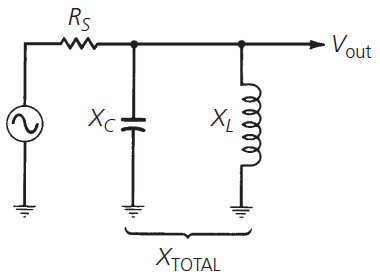
\includegraphics[width=0.5\linewidth]{graphics/22.png}
	\caption{Resonant circuit with two reactive components.}
	\label{fig:22}
\end{figure}

\subsubsection{Loaded Q}
\begin{itemize}
	\item \textit{Q} - The ratio of the center frequency of the resonant
	circuit to its bandwidth is defined as the circuit Q.
	\item The higher its Q, the narrower its bandwidth.
\end{itemize}
\begin{equation}
Q = \dfrac{f_e}{f_2-f_1}
\end{equation}

\begin{figure} [H]
	\centering
	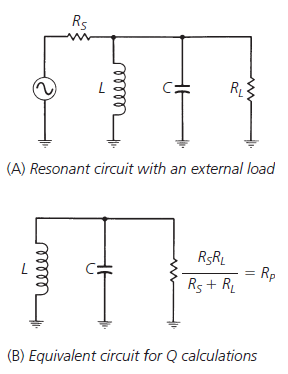
\includegraphics[width=0.5\linewidth]{graphics/24.png}
	\caption{Equivalent parallel impedance across a resonant circuit.}
	\label{fig:24}
\end{figure}

\begin{equation}
Q_p = \dfrac{R_p}{X_p}
\end{equation}

\begin{equation}
Q_s = \dfrac{X_s}{R_s}
\end{equation}

\begin{description}
	\item[$R_p$] equivalent parallel resistance of $R_s$ and $R_L$
	\item[$X_p$] inductive or capacitive reactance (equal at resonance)
\end{description}

\noindent\textit{The optimum Q of a resonant circuit is obtained when the inductor
	is a \textbf{small value} and the capacitor is a \textbf{large value}.}
\newpage
\begin{itemize}
	\item Two approaches to follow in designing a resonant circuit with a particular \textit{Q}
	\begin{itemize}
		\item Select an optimum value of source and load impedance
		\item Select component values of \textit{L} and \textit{C} that	optimize \textit{Q}
	\end{itemize}
\end{itemize}

\subsubsection{Series-to-Parallel Transformation}
Prior assumed that the components used in the resonant circuits are lossless. Due to component losses, there exists some finite equivalent parallel resistance.\\

\noindent Transformation Equation

\begin{equation}
R_p = (Q^2 +1)R_s
\end{equation}

\begin{description}
	\item[$R_p$] equivalent parallel resistance
	\item[$R_s$] series resistance of the component
	\item[$Q = Q_s$] which equals $Q_p$ which equals the \textit{Q} of the component
	\item[$X_p = \dfrac{R_p}{Q_p}$]
\end{description}

\noindent If \textit{Q} of the component is greater than 10, then,
\begin{equation}
R_p \approx Q^2 R_s
\end{equation}

\noindent and

\begin{equation}
X_p \approx X_s
\end{equation}
\begin{figure} [H]
	\centering
	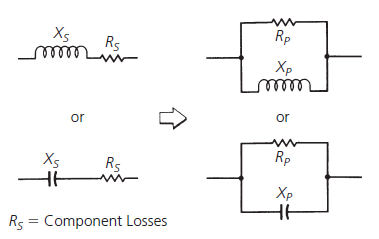
\includegraphics[width=0.5\linewidth]{graphics/23.png}
	\caption{Series-to-parallel transformation.}
\end{figure}
\newpage
\subsubsection{Impedans transformation}
\begin{itemize}
	\item Impedance transforming circuits
\end{itemize}

\begin{figure} [H]
	\centering
	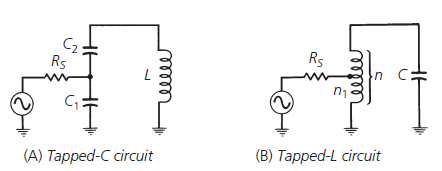
\includegraphics[width=0.8\linewidth]{graphics/25.png}
	\caption{Equivalent parallel impedance across a resonant circuit.}
	\label{fig:25}
\end{figure}

\begin{itemize}
	\item Tapped-C transformer
\end{itemize}

\begin{equation}
R'_s = R_s \left(1+\dfrac{C_1}{C_2}\right)^2
\end{equation}

\begin{itemize}
	\item Equivalent capacitance $C_T$ will resonate with the inductor ($C_1$ in series with $C_2$)
\end{itemize}

\begin{equation}
C_T=\dfrac{C_1 C_2}{C_1+C_2}
\end{equation}

\begin{itemize}
	\item Tapped-L network
\end{itemize}

\begin{equation}
R'_s = R_s \left(\dfrac{n}{n_1}\right)^2
\end{equation}


\subsection{Filter design}
\begin{itemize}
	\item Resonant frequency
\end{itemize}

\begin{equation}
F_r=\dfrac{1}{2\pi\sqrt{L C}}
\end{equation}

\subsection{Frekvens og impedans skalering}